%\documentclass[12pt,a4paper,titlepage]{report}
%\documentclass[a4paper,twoside]{article} 
%\documentclass[12pt,a4paper,twoside]{article} 

%\documentclass[xetex,mathserif,serif,titlepage,a4paper]{article}

\documentclass[xetex,12pt,a4paper]{report}

%\usepackage[xetex,draft]{graphicx}
\usepackage[xetex]{graphicx}

\usepackage[english]{babel}

\usepackage[pdftex,
	% remove to generate the printout version
	colorlinks=true,
	citecolor=black,
	urlcolor=black
	pdfauthor={Andreas Reufer},
	pdftitle={Collisions and impacts in planetary system},
	pdfkeywords={SPH, computational astrophysics, rocket science}]{hyperref}


\usepackage{amssymb}
\usepackage{amsmath}
\usepackage{mathrsfs}
\usepackage{amsfonts}
\usepackage{pdfpages}

\usepackage{algorithmic}
\usepackage{algorithm}

\usepackage{multirow}

\footnotesep0.5cm

%% One and a half spacing
\usepackage{setspace}

\usepackage{a4wide}
\usepackage{enumerate}

\usepackage{natbib}
\usepackage{chapterbib}
\bibpunct{(}{)}{;}{a}{}{,}

\usepackage{verbatim}
\usepackage{moreverb}
\usepackage{fontspec}
\usepackage{xltxtra}

%--------------
% Use the fancyhdr-package and redefine headings, page numbers, etc.
\usepackage{fancyhdr}
% Use the pagestyle of this package
\pagestyle{fancy}
% Redefine the mark for the even side: chapternumber + chaptername in uppercase letters
\renewcommand{\chaptermark}[1]{\markboth{#1}{}}
% Redefine the mark for the odd side: sectionnumber + sectionname in uppercase letters
\renewcommand{\sectionmark}[1]{\markright{#1}{}}
% Clear all headings
\fancyhf{}
% Pagenumber on the left of even and on the right of odd pages
\fancyhead[LE,RO]{\thepage}
% Chapter on the right of even pages
\fancyhead[RE]{\leftmark}
% Section on the left of odd pages
\fancyhead[LO]{\rightmark}
% Draw line below heading
\renewcommand{\headrulewidth}{0.5pt}
% No footer, no line at the bottom of the page
\renewcommand{\footrulewidth}{0pt}
% Redefine pagestyle 'plain' for starting chapters: all empty
\fancypagestyle{plain}{\fancyhead{}\renewcommand{\headrulewidth}{0pt}}
% Incrase height of head a little bit
\addtolength{\headheight}{2pt}
% End of fancyhdr-Definitions
%--------------

% Use the xspace package to provide a space after user defined abbreviations if one is necessary
% (if a word follows) and to supress the space at the end of the sentence. See the definition of \COO below.
\usepackage{xspace}

% Use the booktabs package to make nice lines in tables
\usepackage{booktabs}

% Use the package caption2 for captions in smaller font
\usepackage[footnotesize]{caption}

% Use the package flafter to make sure floating objects appear after their declaration in the text
\usepackage{flafter}

% \linespread{1.6}

% \clearemptydoublepage: start a new page on the right side of the book (odd page number).
% Used before the \chapter command and in similar cases
\newcommand*{\clearemptydoublepage}{\newpage{\pagestyle{empty}\cleardoublepage}}%

% ability to make single landscape pages
\usepackage{lscape}

\usepackage{aux/aas_macros}

% abbreviations
\def\SSC{\textsc{ssc}~}

% mathematical symbols
\def\rv{\boldsymbol{r}}
\def\rvij{\boldsymbol{r}_{ij}}
\def\rvi{\boldsymbol{r}_{i}}
\def\rvj{\boldsymbol{r}_{j}}
\def\rvs{\boldsymbol{r}'}
\def\ud{\boldsymbol{d}}
\def\Xv{\boldsymbol{X}}

\def\d{\mathrm{d}}

\def\vv{\boldsymbol{v}}
\def\vvij{\boldsymbol{v}_{ij}}

\def\av{\boldsymbol{a}}
\def\ev{\boldsymbol{e}}


\def\Lagr{\mathcal{L}}
\def\deg{^\circ}

% SPH stuff
\def\Wij{W_{ij}}
\def\dWij{\nabla W_{ij}}
\def\limhzero{ \lim_{h \to 0}}
\def\d{\partial}

\def\it{\textit}

% physics stuff
%\def\ME{M_{Earth}}
%\def\ME{M_{\earth}}
\def\ME{M_{\oplus}}
\def\ML{M_{\leftmoon}}

\def\RE{R_{\oplus}}

\def\wtp{ wt\mathrm{\%} }
\def\silc{\mathrm{SiO}_2}
\def\watr{\mathrm{H}_2 \mathrm{O} } 
\def\iron{\mathrm{Fe}}

% collision stuff
\def\thimp{\theta_{imp}}
\def\Thimp{\Theta_{imp}}
\def\thgraz{\theta_{graz} }

\def\Mimp{M_{imp}}
\def\Mtar{M_{targ}}
\def\Mlr{M_{lr}}
\def\Msr{M_{sr}}
\def\Mtot{M_{tot}}

\def\Rimp{R_{imp}}
\def\Rtar{R_{targ}}
\def\vimp{v_{imp}}
\def\vesc{v_{esc}}
\def\vinf{v_{+\infty}}
\def\vneginf{v_{-\infty}}
\def\vcr{v_{cr}}

\def\tcol{t_{col}}

\def\rss{\emph{r3} }
\def\css{\emph{c1} }
\def\iss{\emph{i1} }





\let\verbatiminclude\verbatimtabinput
\def\verbatimtabsize{4\relax}


\fontspec [ Path = ./fonts/, 
BoldFont	= MinionPro-Bold.otf ,
ItalicFont	= MinionPro-It.otf ,
BoldItalicFont = MinionPro-BoldIt.otf ] {MinionPro-Regular.otf}

%\fontspec [ Path = ./fonts/, 
%BoldFont	= FrutigerLTStd-Bold.otf ,
%ItalicFont	= FrutigerLTStd-LightItalic.otf ,
%BoldItalicFont = FrutigerLTStd-BoldItalic.otf ] {FrutigerLTStd-Light.otf}

\setromanfont{Minion Pro}
%\setsansfont{Frutiger LT Std}
%\setsansfont{Gill Sans}


\begin{document}
\pagestyle{headings}
%\begin{spacing}{1.5}
\begin{spacing}{1.0}
%\begin{spacing}{1.2}

%% Sections

%\pagestyle{empty}

\begin{titlepage}
\begin{center}

\textbf{ \vspace{3.0cm} \\ \Huge Collisions in planetary systems } \\ \vspace{2.0cm}
\large{ Inauguraldissertation \\ der Philosophisch-naturwissenschaftlichen Fakultät \\ der Universtät Bern } \\ \vspace{3.0cm}
\large{ vorgelegt von} \\ \vspace{0.3cm}
\textbf{ \LARGE Andreas Reufer } \\ \vspace{0.3cm}
\large{ von Flawil SG } \\ \vspace{3.0cm}
\large{ Leiter der Arbeit \\ Prof. Dr. W. Benz \\ Physikalisches Institut der Universtät Bern} 

\clearpage

\textbf{ \vspace{0.0cm} \\ \Huge Collisions in planetary systems } \\ \vspace{2.0cm}
\large{ Inauguraldissertation \\ der Philosophisch-naturwissenschaftlichen Fakultät \\ der Universtät Bern } \\ \vspace{2.5cm}
\large{ vorgelegt von} \\ \vspace{0.3cm}
\textbf{ \LARGE Andreas Reufer } \\ \vspace{0.3cm}
\large{ von Flawil SG } \\ \vspace{2.5cm}
\large{ Leiter der Arbeit \\ Prof. Dr. W. Benz \\ Physikalisches Institut der Universtät Bern} \\ \vspace{2.5cm}
\large{ Von der Philosophisch-naturwissenschaftlichen Fakultät angenommen. } \\ 
\begin{flushleft}Bern, 29.9.2011 \hspace{7.0cm} Der Dekan \\
\hspace{10.25cm} Prof. Dr. Silvio Decurtins\\ \end{flushleft}

\end{center}
\end{titlepage}

\cleardoublepage

\title{Collisions in planetary systems}
\author{Andreas Reufer}
\date{\today}

\tableofcontents
%\listoffigures
%\listoftables
%%\cleardoublepage

\begin{figure}
\begin{center}
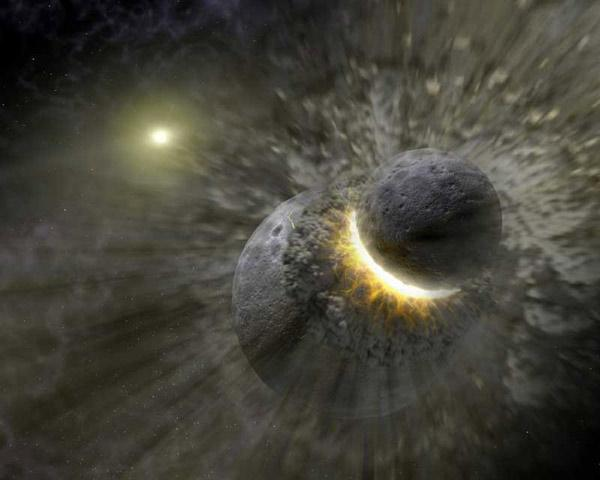
\includegraphics[scale=0.6]{01figs/01planet-collision.jpg}
\caption{Artists impression of the Moon forming giant impact. Image courtesy of NASA/JPL-Caltech}
\label{ch01_fig01}
\end{center}
\end{figure}


\chapter{Introduction}
\label{ch01}
\graphicspath{{./01figs/}}
Collisions between bodies of various sizes are an important process during all stages of planet formation. A collision consists of two macroscopic bodies, the larger body termed the \emph{target} and the smaller body the \emph{impactor} approaching each other and resulting in a collisional outcome depending on various parameters. When the target is considerably larger than the impactor, a collision is also often called an impact. Collisions occur at various stages during planet formation, with mass and size ranges of the involved bodies varying several tens of magnitudes from dust grains up to Jupiter sized planets. This thesis covers different types of collisions all modeled with the same type of method described in detail in chapter \ref{ch02}. The following brief overview of planet formation helps in putting these different types of collisions in context.

The field of planet formation lead a neglected existence besides related fields like stellar formation or cosmology for a long time. While telescopes allowed mankind to observe stars beyond the solar system for several centuries, the knowledge about planets has long been limited to the ones in our own system. The relative small luminosity of planets compared to stars makes it even today almost impossible to directly detect planets even for stars in our neighborhood. Without any further known systems, the question wether planet formation is a common process alongside of stellar formation remained non answerable question. But the common wisdom was, that the solar system is a typical result of planet formation and that hypothetical extrasolar systems should look similarly. This is no surprise, as planet formation models primarily aimed at explaining the solar system.

The discovery of the first extrasolar planet \emph{51 Pegasi b} around a solar-type star by \cite{1995Natur.378..355M} caused an overnight revolution in the field. 
Before this discovery, nobody deemed it possible that a Jupiter-mass planet could exist as close as $0.05 AU$ to its host star. As of July 2011, ongoing ground- and space-based observations have discovered more than 560 extrasolar planets. All of them are relatively massive and close-in, more resembling the originally observed \emph{51 Pegasi b} than the planets in our own solar system. This is primarily an effect of observational bias, favoring the detection of massive, close-in planets. Nevertheless, a model of planet formation also has to explain those systems.

According to the current understanding of planet formation, the formation process of a planetary system can be divided into different stages: A part of a giant molecular cloud, composed of gas (mainly H \& He) and dust, collapses and starts to form a rotating disk due to the conservation of angular momentum. When density and pressure are large enough in the center, hydrogen burning starts and a new star is born. What resembles more a rotating lump of gas at first, changes over time into a disk with decreasing pressure, density and temperature as a function of the distance to the star. This happens over a timescale of $\approx 10^5$ years.


Due to the radial pressure gradient, the gas in the disk rotates with a sub-keplerian velocity around the star. In the vertical direction of the disk, there is also a positive pressure gradient towards the midplane. While the dust is tightly coupled to the rotation of the gas around the star, it is pressureless in itself and therefore settles towards the disks midplane over a timescale of $10^4$ years. The $\mu m$-sized dust starts to coagulate due to strong van-der-Waals forces into larger grains \citep{2010A&A...513A..56G}. As the grains grow towards bigger planetesimals their relative strength decreases as inter-molecular forces increase $\sim r^2$ while intertial forces increase with $\sim r^3$. With the diameter approaching the \emph{meter-sized barrier}, further growth of the solid bodies is stopped \citep{Benz1999Icar..142....5B}.

How this barrier can be overcome is still unknown. Recent suggestions have been the trapping of dust in vortices, either caused by magneto-rotational-instability \citep{Johansen:2007p37} or by turbulence in general \citep{2008ApJ...686.1292I}. In those scenarios, the trapped dust instantly collapses under its own self-gravity into \emph{Ceres} sized objects ($\approx 10^{-4} \ME$). In this regime, gravity becomes strong enough to hold together those objects and further mass is accreted. Due to gravitational focussing, the zone where those bodies accreted mass from increases along with their mass and leads to \emph{runaway accretion}. During this stage, the amout of gas in the disk already has decreased, either by accretion onto the central star or due to photo-evaporation due to the young stars UV radiation. After $\approx 10$ million years, the gas has largely disappeared.

The growing planetesimals now turn into planetary embryos and become a victim of their own success: When an embryo reaches a mass roughly $ 100\times$ larger than the typical planetesimal mass in its vicinity, this feeding zone is being emptied and the accretion rate goes down again. Neighboring embryos can catch up and the \emph{oligarchic} accretion regime kicks in \citep{1993Icar..106..210I, 2010ApJ...714L.103O}.

During oligarchic growth, the individual embryos obtain similar masses and are orderly spaced according to their feeding-zones. The remaining small planetesimals stabilize the orbits of the embryos through dynamical friction, while their own eccentricities and inclinations are pumped up. This leads to a slow removal of the small planetesimals due to accretion onto embryos, loss into the central star or due to ejection. Without the planetesimals and with almost no gas around, the embryos becomes unstable again and eventually get on crossing orbits. The resulting two-body interactions chaotically re-arrange the embryos in the disk and also lead to collisions of embryos \cite{Chambers:2001p2105, Chambers:2004p4098}. With all embryos occupying the same mass regime, these collisions are called similar-sized and lead to various outcomes \cite{Asphaug:2010p3539}. Such collisions and their outcomes are discussed in detail in chapter \ref{ch03}. Work on modeling the stage between the formation embryos and their final accretion into proto-planets \citep{Chambers:2001p2105, 2006Icar..184...39O} often makes simplified assumptions about these similar-sized collisions. The data provided in chapter \ref{ch03} permits such models to incorporate a more realistic collision handling and to model this stage of planet formation more accurately.

Similar-sized collisions alter bodies in a profound way: Properties like composition, bulk density \citep{Benz:1988p3336} or the rotation can be changed by this collisions. They are also believed to trigger core formation \citep{1992Icar..100..326T}. Consequently, the final properties of terrestrial planets are heavily influenced by the last massive collision they underwent: Primordial atmospheres can be removed \citep{2002DPS....34.2804A} or the planet can be depleted of its volatiles \citep{2001E&PSL.192..545H}.

Another interesting effect of such collisions is satellite formation. Along with the Pluto-Charon binary system \citep{Canup:2005p1987}, the Earths Moon is most probably a direct outcome of a late giant collision between the proto-Earth and a roughly Mars sized body \citep{1975Icar...24..504H, 1976LPI.....7..120C, 1987Icar...71...30B, Canup:2001p1861}. In chapter \ref{ch05}, we look into a model explaining the Moons formation with an alternative impact scenario.

The growth of solid embryos is not only important for the formation of terrestrial planet, but also delivers the cores required for giant planet formation \citep{1996Icar..124...62P}. Understanding the timescales of embryo growth is crucial, as they have to becomes massive enough to start to accrete gas, before the gas disk vanishes. 

With the late heavy bombardment marking the last major event in the solar systems history \citep{2005Natur.435..466G}, planet formation as a process has finished. Nevertheless, impacts of small remnants for example from the asteroid or the Kuiper belt onto planets and their moons still take place. While not delivering substantial mass relative to the target body, the craters such impacts leave give clues about the rheology and age of planetary surfaces. Chapter \ref{ch04} presents modeling work on martian craters which have been observed only months after their formation \cite{2009Sci...325.1674B}. 

give outlook with future missions



%statistical results for evolution codes, to understand planet formation in general 

especially terrestrial planet formation 
%\cite{Lisse:2009p3131} -> chapter 3

cratering collisions: helpful for dating 
application of impacts mars -> chapter 4


method side: SPH as a robust method for collisions, thermodynamics are important

%SPH has been used for single, large cases mainly \cite{2005Natur.435..629S}

progress in computational methods and computing power allows massively parallel 




%\section{Motivation}
%collisions as event between two bodies
%cratering to similar sized collisions
%importance in solar system formation
%outcomes give clues 
%solar system dimensions
% refer to chapters: 

% motivation for simulating collisions
% introduce collision basics and terms
% give examples of collisions

% check Augustins Diss

%\section{Collision basics}
%introduce terms: impactor, target, impact velocity, impact angle

\bibliographystyle{plainnat}
%\bibliographystyle{nabstract}
\bibliography{bibliography}

\graphicspath{{./02figs/}}

\tableofcontents

\chapter{Methods}
Collision events are characterised by a 
range of dynamical 

%\subsection*{Introduction}
%\includepdf[pages={2-},fitpaper=true]{/tree_musings}

Motivation to use SPH, spatial dynamics of collisions, SPH particles are where the mass is (not entirely true for collisions, but necessary), free boundaries



Lagrangian nature vs. grid techniques, complexity of AMR vs. simplicity of SPH

Neighbour search is the hardest thing about SPH



In this chapter we will discuss, how collisions in the strengthless regime as appearing in planetary systems can be modelled.
The first section gives a short review the governing physics of such collisions and will provide us with a closed set of equations, namely the Navier-Stokes equations and the 
This set is far too complicated to be solved in an analytical way. 
Smoothed particle Hydrodynamics (SPH) is a method which discretises fluids with particles of finite volume and presents a framework to solve the equations describing the fluid.
The second section derives different SPH formulations of the Navier-Stokes equations and demonstrates the advantages and disadvantages of each formulation.

gravity section: 

The initial conditions and also the outcome of collisional events can be charaterized by a 

Smoothed particle hydrodynamics (SPH) is a numerical method which can discretize 

(insert a nice picture of equations, code lines and numbers here)

\newpage

\section{Fluid- and Thermodynamics}
A continuum model 


%%
%   F L U I D S
%%
\subsection{Theory of Fluids}

\begin{equation}
\label{ch02_fld01_eq001}
\frac{\partial \rho}{\partial t} + \rho \nabla \mathbf{v} = 0
\end{equation}

\begin{equation}
\label{ch02_fld01_eq002}
\rho \frac{\partial \mathbf{v}}{\partial t} + \rho ( \mathbf{v} \nabla ) \mathbf{v} = - \nabla p + \eta \Delta \mathbf{v} + ( \zeta + \eta ) \nabla ( \nabla \mathbf{v} )
\end{equation}

\label{ch02_fld01_eq003}
\begin{equation}
- \frac{\partial \mathbf{v}}{\partial t} =  ( \mathbf{v} \nabla ) \mathbf{v} + \frac{\nabla p}{\rho}
\end{equation}

The Lagrangian of a inviscous fluid is given by
\begin{equation}
\label{ch02_fld01_eq004}
\Lagr = \int \Big( \frac{1}{2} \rho \vv ^2 - \rho u \Big) dV
\end{equation}

\cite{Thorne:2008}

%%
%   S P H
%%

% todo: mention SPH limit
\subsection{SPH formalism}
The basic idea of SPH is to interpolate all continuum variables in space with an interpolant.
If our variable is $A(\rv)$ defined at all points in space $\rv$, we start with the basic equality

\begin{equation}
\label{ch02_sph01_eq001}
A(\rv) = \int  \delta(\rv - \rvs) A(\rvs) \ud \rvs
\end{equation}

We now replace the $\delta$-function with a smoothing kernel $W$, which has typical width $h$, the smoothing length, and which fulfils the following two criteria

\begin{equation}
\label{ch02_sph01_eq002}
\limhzero W(\rv - \rvs, h) = \delta(\rv - \rvs) \hspace{1.0cm}
\int W(\rv - \rvs, h) \ud \rvs = 1
\end{equation}

Equation \ref{ch02_sph01_eq001} can now be re-written as 

\begin{equation}
\label{ch02_sph01_eq003}
A(\rv) = \int  W(\rv - \rvs, h) A(\rvs) \ud \rvs + O(h^2)
\end{equation}

The variable $A(\rv)$ is now smoothed out over the characteristic scale $h$. By replacing the $delta$-function with a kernel of finite length, an error in the order of $h^2$ is introduced. Now comes the particle part: The continuum is replaced by a finite set of points (\emph{particles}), on which the quantities are defined. The integral can now be replaced by a sum with a finite number of summands:

\begin{equation}
\label{ch02_sph01_eq004}
A(\rv) \approx \sum_{j} W(\rv - \rvj) A_i V_{j} \hspace{1.0cm} V_{j} = \frac{m_j}{\rho_j}
\end{equation}

$V_{j}$ is the particle volume and is usually given assigning each particle a mass and dividing it by the density. The particles used in the summation are called \emph{neighbours} and are indexed here with $j$. For most purposes, the variable only needs to be known at particle position $i$. For convenience, we write the kernel used between two particles as $\Wij = W( \rvi - \rvj, h)$\\

Spatial derivatives are easily given by taking the partial derivative of the integral interpolant variable and replacing it again by the sum over all neighbours:

\begin{equation}
\label{ch02_sph01_eq005}
\nabla A(\rv_i) = \frac{\partial}{\partial \rv}\int A(\rvs) \ud \rvs \frac{\partial}{\partial \rv}\ W(\rv_i - \rvs, h) + O(h^2)
\approx \sum_{j} A_j V_{j} \nabla \Wij 
\end{equation}

Rotations of variables can be similarly obtained:
\begin{equation}
\label{ch02_sph01_eq006}
\nabla \times A_i \approx \sum_{j} A_i V_{j} (\nabla \times \Wij)
\end{equation}

Like in in grid based schemes, there are different ways of calculating spatial derivatives in SPH.
Depending on the actual application of the derivative, whether it is to get the velocity divergence or a pressure gradient, there are better suited variants which show better error behaviour. They will be presented shortly.

The kernel has to fulfill the two constraints posed by equations \ref{ch02_sph01_eq002}. A natural choice would be a normalized Gaussian, but this has the unpleasant of never vanishing. All particles, also distant ones, would contribute to every individual SPH sum, making the method very inefficient. A better choice are therefore functions with compact support: Functions which vanish at sufficiently large distances. A common selection are cubic splines

\begin{equation}
\label{ch02_sph01_eq007}
W(| \rv |, h) = \frac{\sigma}{h^\nu \pi} \left \{ \begin{array}{lll}
1 - \frac{3}{2}q^2 + \frac{3}{4}q^3 & r \leq h & \\
\frac{1}{4}(2-q)^3 & h < r  \leq 2h & \hspace{1.0cm} q = r / h\\
0 & 2h < r & \\
\end{array} \right. 
\end{equation}

where $\nu$ stands for the number of spatial dimensions and $\sigma = \big( \frac{2}{3}, \frac{10}{7\pi}, \frac{1}{\pi} \big) $ for $\big( 1,2,3\big)$ dimensions. The Kernel vanishes for distances greater than $2h$, reducing SPH sums to contributing terms of only the nearest neighbours. The first derivative is given by 

\begin{equation}
\label{ch02_sph01_eq008}
\nabla W(\rv, h) = \frac{\rv}{r} \frac{\sigma}{h^\nu \pi} \left \{ \begin{array}{ll}
1 - 3q + \frac{9}{4}q^2 & r \leq h \\
\frac{3}{4}(2-q)^2 & h < r  \leq 2h \\
0 & 2h < r \\
\end{array} \right. 
\end{equation}

and is also continuous. 

\subsection{standard SPH}
The original and most widely used version of SPH uses the density and particle mass to calculate the particle volumes ($V_j = m_j / \rho_j)$ and the density to interpolate all variables. The density is given by the simple particle sum

\begin{equation}
\label{ch02_sph02_eq001}
\rho_i = \sum_{j} m_j \Wij
\end{equation}

The velocity divergence $\nabla \vv$ could in principle be written as
\begin{equation}
\label{ch02_sph02_eq002}
\nabla \vv_i = \sum_{j} \frac{m_j}{\rho_j} \vv_j \nabla \Wij
\end{equation}

but this form has the disadvantage of being asymmetric and will ultimately lead to a non-conservative form for the linear momentum. It is better to apply the \emph{second golden rule} of SPH \citep{Monaghan:1992p3721} to re-write the velocity divergence term with the density placed inside the operators:

\begin{equation}
\label{ch02_sph02_eq003}
\nabla \vv = \frac{1}{\rho} \Big( \nabla (\rho \vv) - \vv \nabla \rho \Big)
\end{equation}

so that the corresponding SPH sum becomes 

\begin{equation}
\label{ch02_sph02_eq003}
\nabla \vv_i = \frac{1}{\rho_i} \sum_{j} \frac{m_j}{\rho_j} \rho_j \vv_j \Wij - \frac{1}{\rho_i} \vv_i \sum_{j} \frac{m_j}{\rho_j} \rho_j = \frac{1}{\rho_i} \sum_{j} m_j \vvij \Wij 
\end{equation}

with $\vvij = \vv_j - \vv_i$, which is a symmetric form for the velocity divergence. If we take the partial time derivative of \ref{ch02_sph02_eq001}, where only the particle positions in the Kernel depend explicitly on time, we get: 

\begin{equation}
\label{ch02_sph02_eq004}
\frac{\partial \rho_i}{\partial t}  = \sum_{j} m_j \Big( \frac{\partial}{\partial t} \rvij \Big) \nabla \Wij = \sum_{j} m_j \vvij \nabla \Wij 
\end{equation}

So this equation together with the velocity divergence equation \ref{ch02_sph02_eq003} fulfills the continuity equation \ref{ch02_fld01_eq001} for each particle.

The equations of motion can be derived in two different ways: With the inviscous equation of motion of the Navier-Stokes equation \ref{ch02_fld01_eq003}, a symmetric formulation for the pressure gradient term $\nabla p / \rho$ can be found with the trick used above for the velocity divergence. 
A more elegant way is to derive the equation of motion directly from the Lagrangian given by equation \ref{ch02_fld01_eq004}, whose SPH formulation is

\begin{equation}
\label{ch02_sph02_eq004}
\Lagr = \sum_{j} m_j \Big( \frac{1}{2} \vv_j^2 - u(\rho_j, s_j) \Big) 
\end{equation}

where $u$ is the specific internal energy of a fluid particle dependent only on its density and specific entropy $s$. The Euler-Lagrange equations for a single particle $i$ is

\begin{equation}
\label{ch02_sph02_eq005}
\frac{d}{dt} \Big( \frac{\partial \Lagr}{\partial \vv_i} \Big) - \frac{\partial \Lagr}{\partial \rv_i} = 0
\end{equation}

which yields 

\begin{equation}
\label{ch02_sph02_eq006}
m_i \frac{d \vv_i }{dt} = \sum_{j} m_j \frac{\partial u_j}{\partial \rho_j} \frac{\partial \rho_j}{\partial \rv_i}
\end{equation}

for constant entropy, which is the case in the absence of shocks. The first law of thermodynamics for a particle is given by

\begin{equation}
\label{ch02_sph02_eq007}
\frac{u_j}{\rho_j} = \frac{p_j}{\rho_j^2}
\end{equation}

and the divergence of the density is directly given by

\begin{equation}
\label{ch02_sph02_eq008}
\frac{\partial }{\partial \rv_i} \rho_j
= \sum_{k} m_k \frac{\partial}{\rv_i} W_{jk} 
= \sum_{k} m_k \nabla W_{jk} ( \delta_{ji} - \delta_{ki})
\end{equation}

where the kernel vanishes except if $i = j$ and if $i = k$. So equation \ref{ch02_sph02_eq006} yields

\begin{equation}
\label{ch02_sph02_eq009}
m_i \frac{d \vv_i }{dt} = \sum_{j} m_j \frac{p_j}{\rho_j^2} \sum_{k} \nabla_i W_{jk} ( \delta_{ji} - \delta_{ki})\\
 = m_i \sum_{j} m_j \Big( \frac{p_i}{\rho_i^2} + \frac{p_j}{\rho_j^2} \Big) \nabla W_{ij}
\end{equation}

and leaves us with a symmetric SPH sum for the acceleration of a particle in absence of shocks:
\begin{equation}
\label{ch02_sph02_eq010}
\frac{d \vv_i }{dt} = \sum_{j} m_j \Big( \frac{p_i}{\rho_i^2} + \frac{p_j}{\rho_j^2} \Big) \nabla W_{ij}
\end{equation}

The derivative of the kernel is anti-symmetric ($\nabla W_{ij} = - \nabla W_{jj}$), therefore each interacting particle pair fulfils Newtons third law \emph{actio-reactio} and linear momentum is conserved. Angular momentum is also conserved, which can be shown by taking the time derivative of the $\frac{d}{dt} \sum_i (m_i \rv_i \times \vv_i)$ where some index magic \citep{Price:2004p2613} again shows that all terms cancel each other out in the sum over all particles.

In most cases, the internal enery of the fluid is non-constant, so we also need a equation for the change in internal energy due to compressional heating.
The rate of change in specific internal energy is given by 

\begin{equation}
\label{ch02_sph02_eq011}
\frac{du}{dt} = -\frac{p}{\rho} \nabla \vv
\end{equation}

Using the velocity divergence SPH sum \ref{ch02_sph02_eq003}  yields

\begin{equation}
\label{ch02_sph02_eq012}
\frac{du_i}{dt} = \frac{p_i}{\rho_i^2} \sum_{j} m_j \vvij  \dWij
\end{equation}

An SPH sum of this equation consistent with the equation of motion from above can be obtained by applying the golden rule again and putting the density inside the divergence operators:

\begin{equation}
\label{ch02_sph02_eq013}
\frac{du}{dt} = - \nabla \Big( \frac{p \vv}{\rho} \Big) + \vv \nabla \Big( \frac{p}{\rho} \Big)
\end{equation}

The corresponding SPH sum yields the asymmetric equation

\begin{equation}
\label{ch02_sph02_eq014}
\frac{du_i}{dt} = - \sum_{j} m_{j} \frac{p_j \vv_j}{\rho_j} \dWij + \vv_i \sum_{j} m_{j} \frac{p_j}{\rho_j^2}  \dWij = \sum_{j} m_j \vvij \frac{p_j}{\rho_j^2}  \dWij
\end{equation}

A symmetric formulation can be gained by taking the average of equations \ref{ch02_sph02_eq012} and \ref{ch02_sph02_eq014}:

\begin{equation}
\label{ch02_sph02_eq015}
\frac{du_i}{dt} = \frac{1}{2} \sum_{j} m_{j} \vvij \Big( \frac{p_i}{\rho_i^2}  + \frac{p_j}{\rho_j^2} \Big) \dWij
\end{equation}

\subsection{Resolving shocks}
Shocks are changes of the characteristics of a fluid on the spatial scale of the molecules mean-free path. Discontinuities arise in the fluid approximation, usually in density, pressure and temperature.
Numerical schemes tend to react to these discontinuities with unphysical oscillations behind the shock front, because the sharp changes cannot be resolved properly.
Several approaches exist to tackle this problem. Godunov-schemes solve the Riemann problems on both sides of the shock exactly between computational elements and in a second step superpose all pair-wise solutions for each element. In case of SPH this can be done by solving the Riemann problem for each particle against its neighbours \citep{Monaghan:1997p3938}.
Another approach is the von Neumann and Richtmyer viscosity: By introducing a small amount of viscosity, the \emph{artificial viscosity}, the shock front is smoothed out and the oscillations disappear. This can be implemented in SPH by adding additional terms to the momentum and energy equation. The most common used variant is that given by \citep{Monaghan:1992ARAA..30..543M}:

\begin{equation}
\label{ch02_sph02_eq016}
\frac{d \vv_i }{dt} \Big|_{AV} = \sum_{j} m_j \frac{-\alpha c_{ij} \mu_{ij} + \beta \mu_{ij}^2}{\rho_{ij}} \dWij \hspace{1.0cm} \mu_{ij} = \frac{h \vvij \rvij}{\rvij^2 + 0.01h^2}  \hspace{0.5cm} \mathrm{if}  \hspace{0.5cm} \rvij \vvij < 0
\end{equation}

where $\rho_{ij}$ is the averaged density between two particles and $\mu_{ij}$ is a signal velocity with an order of magnitude of the speed of sound. The artificial viscosity term is only applied in situations of compression, where $\rvij \vvij < 0$. The choice of constants is usually $\alpha = 1$ and $\beta = 2 \alpha$. The $\beta$-term is the actual von Neumann and Richtmyer term and becomes dominant in strong shocks where the velocity difference $\vvij$ between two particles in the shock front becomes large. Momentum conservation is still conserved by the symmetric form of the artificial viscosity term.

The contribution of artificial viscosity to the internal energy can be found by requiring that artificial viscosity itself should be energy conserving. The specific energy change due to the dissipative is given by

\begin{equation}
\label{ch02_sph02_eq017}
\frac{de_i}{dt} \Big|_{AV}  = \frac{du_i}{dt}  \Big|_{AV} + \vv_i \frac{d\vv_i}{dt}  \Big|_{AV} = 0
\end{equation}

and should be zero. This leads to the thermal contribution

\begin{equation}
\label{ch02_sph02_eq018}
\frac{du_i }{dt} \Big|_{AV} = - \sum_{j} m_j \vvij \frac{-\alpha c_{ij} \mu_{ij} + \beta \mu_{ij}^2}{\rho_{ij}} \dWij
\end{equation}

with the same choice for the signal velocity $\mu_{ij}$ and numerical constants as in equation \ref{ch02_sph02_eq016}. 

A disadvantage of this approach is that this viscosity also acts outside of shocks in situations of weak compression or shear flows. There exist several approaches to fix this issue by detecting shocks more cleverly \citep{Morris1997J.-Comput.-Phys.Morris} than the simply checking for compression or recognizing shear flows explicitly \citep{Balsara1995JCoPh.121..357B} and suppressing the artificial viscosity in situations where it is not needed. For the simulation of collisions, this is not a big problem, therefore we skip 

\subsection{variable smoothing length}


\subsection{Integration}
Together with an equation of state which gives us the pressure $p_i(u_i, \rho_i)$ and as a side effect also the speed of sound $c_i(u_i, \rho_i)$, we have a closed set of equations describing the fluid which can be integrated in time. A common choice due to its simplicity and low number of derivation steps required is the predictor-corrector scheme \citep{Press2002nrc..book.....P}. For the integration of particle positions we use the second-order form, which yields the prediction step

\begin{eqnarray}
\label{ch02_sph02_eq019}
\rv_i^{(p)} = \rv_i^{(0)} + \frac{1}{2} ( 3 \vv_i^{(0)} - \vv_i^{(-1)} )\Delta t \\
\vv_i^{(p)} = \vv_i^{(0)} + \frac{1}{2} ( 3 \av_i^{(0)} - \av_i^{(-1)} )\Delta t
\end{eqnarray}
and the correction step

\begin{eqnarray}
\label{ch02_sph02_eq020}
\rv_i^{(1)} = \rv_i^{(0)} + \frac{1}{2} ( \vv_i^{(p)} - \vv_i^{(0)} )\Delta t \\
\vv_i^{(1)} = \vv_i^{(0)} + \frac{1}{2} ( \av_i^{(p)} - \av_i^{(0)} )\Delta t
\end{eqnarray}

The integrator requires the evaluation of the derivative $\av_i( \rv_i, \vv_i)$ two times. As the predicted variables $(\rv_i^{(p)}, \vv_i^{(p)})$ and previous variables $(\rv_i^{(-1)}, \vv_i^{(-1)})$ are never used at the same time, it is sufficient to store only one additional set of variables.

Variables defined by first-order differential equations like the internal energy, use the first-order prediction step

\begin{equation}
\label{ch02_sph02_eq021}
u_i^{(p)} = u_i^{(0)} + \frac{1}{2} ( 3 \dot{u}_i^{(0)} - \dot{u}_i^{(-1)} )\Delta t \\
\end{equation}
and the correction step

\begin{equation}
\label{ch02_sph02_eq022}
u_i^{(1)} = u_i^{(0)} + \frac{1}{2} ( \dot{u}_i^{(p)} - \dot{u}_i^{(0)} )\Delta t \\
\end{equation}

The timestep is limited by several factors. Stability analysis of SPH yields the CFL condition 

\begin{equation}
\label{ch02_sph02_eq023}
\Delta t_{CFL} = \mathcal{C}_{CFL} \min_{i} \frac{h_i}{c_i}
\end{equation}

where c is a constant chosen between $\mathcal{C}_{CFL} = 0.1 \dots 0.4$. All other integrated variables require, that the their maximal change per timestep is not more than their own magnitude. In order to avoid arbitrarily small timestep when a variable goes to zero, a minimal value for such quantities is introduced. This yields for example for the smoothing length the timestep

\begin{equation}
\label{ch02_sph02_eq024}
\Delta t_{h} = \mathcal{C} \min_{i} \frac{\dot{h}_i}{h_i + h_{min}}
\end{equation}

Other such variables are specific internal energy $u_i$ or the density $\rho_i$ in case the continuity equation is integrated. 

The predictor-corrector scheme has the disadvantage of a global time step. Other integrators like the leap-frog integrator allows hierarchical time stepping, due to their inherent symmetry of the sub-steps. In most cases the time step is limited by the CFL-criterion \ref{ch02_sph02_eq023}, which depends on the smoothing length and the speed of sound. For an ideal gas at constant entropy and when using particles of a fixed mass, the time step depends on density as 

\begin{equation}
\label{ch02_sph02_eq025}
\Delta t_{CFL} \sim \frac{h}{c} \sim \frac{1}{\sqrt[3]{\rho}} \sqrt{ \frac{\rho}{p} } \sim \frac{1}{\sqrt[3]{\rho}} \frac{1}{\sqrt{u}} \sim \frac{1}{\rho^{2/3}}
\end{equation}

When particle density varies over several orders of magnitudes, so does the time step. This is the case for cosmological simulations, where the collapse of dilute collapse gas to hot dense clumps results in immensely different time steps. Only hierarchical schemes where the actual time steps between derivations are chosen in the same order of magnitude as the required time step allow to integrate such a particle set with reasonable computational effort.
For collision events in the gravity regime, the time steps don't vary too much. Solids have similar speed of sound and smoothing lengths, also under compression. The formation of dilute vapor is not an issue, because particles in vapor state have much larger smoothing lengths than solid length, while retaining a comparable speed of sound, resulting in an even larger time step. A hierarchical time stepping scheme is therefore not necessary for the simulations of collisions.


\subsection{miscible SPH}
Big density contrasts normally arise, when two fluids with different equations of state interact, for example a liquid and a gas in mutual thermal equilibrium. Classical SPH can represent such a situation in two distrinctive ways: Either particle masses are chosen in the same order of magnitude for both fluids, such that the particles densities vary 



Big density contrast present a problem to SPH. 

motivation: big density contrasts
advantages and disadvantages of SPH

\subsection{solid state SPH}

\citep{Nyffeler2004}

integrating density
equations in 
basic problem: stiff equations of state require a non-smooth density 
advantages and disadvantages of SPH


\subsection{ANEOS}
tables, interpolating, iterating, issues\\
show isobars\\
entropy vs. energy integration\\


%%
%   G R A V I T Y 
%%

\citep{Abel:2010p3297}
\citep{Barnes:1986p2853}
\citep{Monaghan:2005p2677}
\citep{Ott:2003p3727}
\citep{Price:2004p2613}
\citep{Solenthaler:2008p3720}
\citep{Springel:2003p3298}
\citep{Monaghan:1992ARAA..30..543M}

% TODO: standard SPH vs. integrated density, surface tension issues, miscible SPH, show m1H vs. m3H\\


\section{Gravity}

\subsection{N-Body problem}

\subsection{Barnes and Hut Tree}


%%
%   I M P L E M E N T A T I O N
%%





\section{Implementation}
\subsection{Organizing particles in Trees}
building a tree\\
deleting a tree\\
neighbour search\\
tree walks\\
accelerating a tree: show skip, next and parent pointers by simple tree examples\\

\begin{figure}[htbp]
\begin{center}
\includegraphics[scale=0.6]{cell_wiring.pdf}
\caption{Wiring scheme of an octree cell node a depth $n$ with particle childs in subvolume 1 and 6 and a cell node as child 3. Parent pointers allow going upwards in the tree, child pointers downwards. Following the next pointers results in a pre-order tree traversal, where taking the \it{skip} pointer skips a cells subtree. Note that a \it{next} pointer }
\label{fig02walks}
\end{center}
\end{figure}


\begin{figure}[htbp]
\begin{center}
\includegraphics[scale=0.6]{orderwalks.pdf}
\caption{Post-order vs. pre-order recursors}
\label{fig02walks}
\end{center}
\end{figure}

\subsection{Tree algorithms}

\subsection{Tree parallelization: shared vs. distributed memory}
intro: shared vs. distributed memory\\

SPHLATCH v1\\
parallelizing a particle code: distributed sums vs. ghosts approach\\
parallelizing a tree\\
show ghost approach\\

disadvantage: distributed memory machines loose importance, not good for parameter space searches, mutlicore machines are the future


SPHLATCH v2\\
shared memory approach\\
load balancing approach, how this could be memory-\\
show cost (gravity, NS, total) for giant impact\\
caching issues\\

building the tree:

mention future of parallel computing: CPU vs. GPU computing, stream computing
trees on GPUs

\section{Tests?}
shocktube
simple gravity tree

\section{Algorithms}
clump detection\\
FOF vs. potential, not parallelized\\
initial conditions: show theoretical vs. unevolved vs. evolved densities, show example of impact with standard SPH and miscible SPH (chondritic, use moon case), setting up a \SSC \\

\subsubsection{Neighbour search}

\subsection{setting up initial conditions}
use of spheres for simplicity reason

\citep{Barnes:1986p2853}
\citep{Monaghan:2005p2677}
\citep{Price:2004p2613}

\bibliographystyle{plainnat}
\bibliography{bibliography}



%\include{03ssc}
%\chapter{Mars impacts}
\label{ch04}
%\includepdf[pages={2-},fitpaper=true]{04figs/f9d1219a0fca0f2cd983b857ca6e3705.pdf}

%\chapter{The giant impact}
\label{ch05}
\graphicspath{{./05figs/}}
haba


%\chapter{Impacts onto proto-Jupiters}

\subsection{putting an atmosphere on top}



% code description
% pmc_colls (paper?)
% fluffy impacts (paper?)
% Mars impacts paper

% Include a bibliography
%\bibliographystyle{plain}
%\bibliographystyle{natbib}
%\bibliographystyle{natdin}
%\bibliographystyle{abbrvnat}
%\bibliographystyle{unsrtnat}

% Appendix
\appendix
%\include{miscappendix}

%\include{acknowledgement}

\end{spacing}
\end{document}
